\documentclass{article}

% Language setting
% Replace `english' with e.g. `spanish' to change the document language
\usepackage[english]{babel}

% Set page size and margins
% Replace `letterpaper' with `a4paper' for UK/EU standard size
\usepackage[letterpaper,top=2cm,bottom=2cm,left=3cm,right=3cm,marginparwidth=1.75cm]{geometry}

% Useful packages
\usepackage{amsmath}
\usepackage{graphicx}
\usepackage[colorlinks=true, allcolors=blue]{hyperref}
\usepackage{float}
\usepackage{matlab-prettifier}
\usepackage{subcaption}
\usepackage{multirow}

\title{Removing Ocular Artifacts using Wavelet Decomposition}
\author{Giacomo Sacco - 899927}

\begin{document}
\maketitle

\section{Comparing fastICA and Wavelet Decomposition}
The goal is to compare the fastICA approach, which is the most common approach in the literature, with a wavelet
transform-based approach for removing ocular artifacts from TMS-EEG data.
The objective is to identify a method that preserves TEP information while eliminating ocular artifacts.

\subsection{Dataset}
\texttt{alberto8\_tdcs\_epoched.set}, which is a raw TMS-EEG dataset, epoched (\texttt{-1000} to \texttt{1000} ms) around the TMS pulse.

\subsection{The pipeline}
The pipeline I used for removing ocular artifacts using wavelet transform is the following:
\begin{enumerate}
    \item Remove unused channels.
    \item Add EOG events to the dataset (optional).
    \item Remove bad channels.
    \item Apply ocular artifacts removal method:
        \begin{enumerate}
            \item fastICA
            \item Wavelet decomposition
        \end{enumerate}
\end{enumerate}
The wavelet decoomposition method is applied on the whole signal, for this reason is not necessary to have the EOG events.

\subsubsection{FastICA}
To apply the fastICA method, the TESA matlab toolbox has been used. 
The following code snippet shows the used parameters and how to apply fastICA for ocular artifact removal:
\begin{lstlisting}[style=Matlab-editor]
    % Highpass filter before ICA (0.1 Hz)
    EEG = pop_tesa_filtbutter( EEG, 0.1, [], 4, 'highpass' ); 

    % fastICA for ocular artifacts
    EEG = pop_tesa_fastica( EEG, 'approach', 'symm', 'g', 'tanh', 'stabilization', 'off' );
    EEG = pop_tesa_compselect(EEG, ...
        'blink','on', ...
        'blinkThresh',2.5, ...
        'blinkFeedback','off', ... 
        'move','on', ...
        'moveThresh',2, ...);
\end{lstlisting}
   
\subsubsection{Wavelet Decomposition}
To remove the ocular artifact has been used a daubechies wavelet 4 (db4) Fig. \ref{fig:db4} with
six levels of decomposition. In order to remove the artifact, the approximation 
coefficients (which is where most of the artifact reside) have been replaced with the mean value of the level.
\begin{figure}[H]
    \centering
    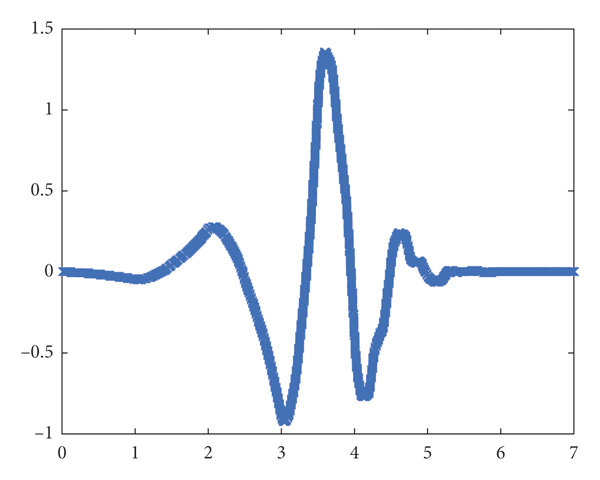
\includegraphics[width=0.2\textwidth]{images/db4.jpg}
    \caption{Real part of the Daubechies wavelet 4 (db4).}
    \label{fig:db4}
\end{figure}

The following code snippet shows how I have applied the method in Matlab:
\begin{lstlisting}[style=Matlab-editor]
%% Wavelet Ocular Artifacts Removal
function EEG = wavelet_OA_rm(EEG)
    levels = 6; % number of levels
    wname = 'db4'; % wavelet name
    for chanIdx = 1:EEG.nbchan
        [c, l] = wavedec(EEG.data(chanIdx, :), levels, wname);
        base_value = mean(c(1:l(1)-1));
        c(1:l(1)-1) = base_value;           
        EEG.data(chanIdx, :) = waverec(c, l, wname);
    end
\end{lstlisting}
\newpage
\subsection{Results}
The results of the comparison between fastICA and wavelet transform in removing ocular 
artifacts.

\subsubsection{Power Spectral Density (PSD) Comparison}
The power spectral density has been calculated on the FP2 channel.
\begin{figure}[H]
    \centering
    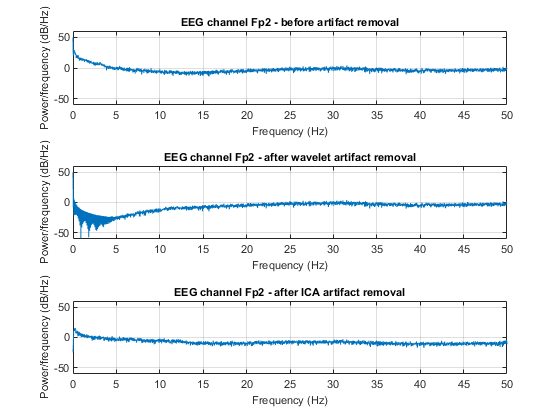
\includegraphics[width=1\textwidth]{images/psd_comparison.png}
    \caption{PSD graphical comparison before and after artifact removal.}
    \label{fig:psd_comparison}
\end{figure}
In order to compare the differences in the power spectral density the \textbf{Root Mean Square Error}
has been calculated, with the following results:
\begin{itemize}
    \item Wavelet vs fastICA: \textbf{40.98} dB/Hz
    \item Wavelet vs original: \textbf{12.93} dB/Hz
    \item fastICA vs original: \textbf{42.45} dB/Hz
\end{itemize}
The results show that the signal after wavelet transform filtering is closer to the orignal, in terms
of frequency content, than the signal after fastICA filtering. 
And the two artifact removal methods have quite different results. 

\subsubsection{Visual Comparison}
In order to visualize in a clearer way the data a bandpass (1-48 Hz) filter was applied.
Figure \ref{fig:37_eegplot} shows raw data with a clear ocular artifacts in epoch 38.
Figure \ref{fig:37_eegplot_ica} shows the channel after fastICA ocular artifact removal, 
while figure \ref{fig:37_eegplot_wavelet} shows the channels after wavelet transform ocular artifact removal.
Both methods show some residual artifacts.

\begin{figure}[htbp]
    \begin{subfigure}{0.33\textwidth}
        \centering
        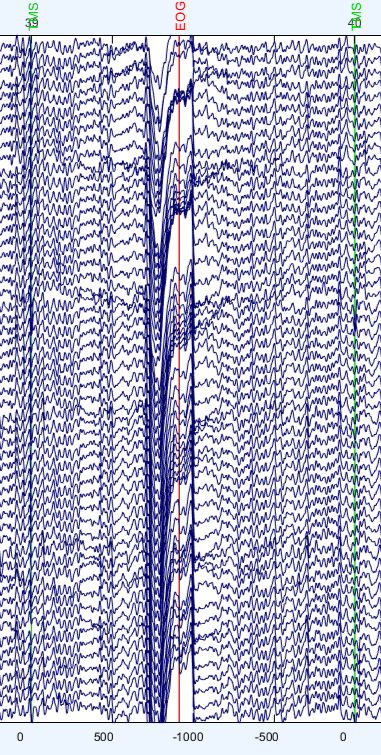
\includegraphics[width=0.9\linewidth, height=10cm]{images/zoom_37eegplot_48hzBP.png}
        \caption{Raw data.}
        \label{fig:37_eegplot}
    \end{subfigure}
    \begin{subfigure}{0.33\textwidth}
        \centering
        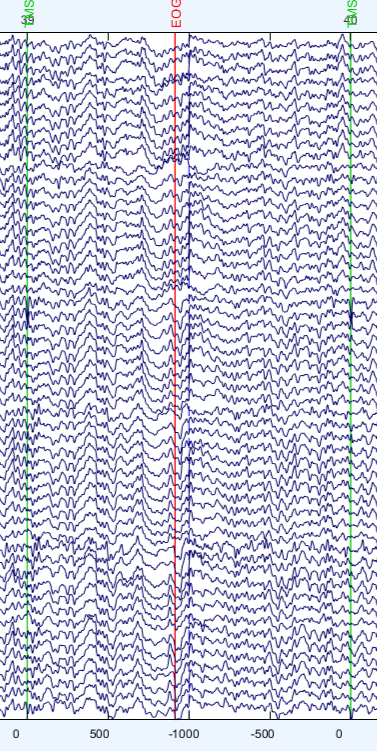
\includegraphics[width=0.9\linewidth, height=10cm]{images/zoom_37eegplot_ica_48hzBP.png}
        \caption{FastICA.}
        \label{fig:37_eegplot_ica}
    \end{subfigure}
    \begin{subfigure}{0.33\textwidth}
        \centering
        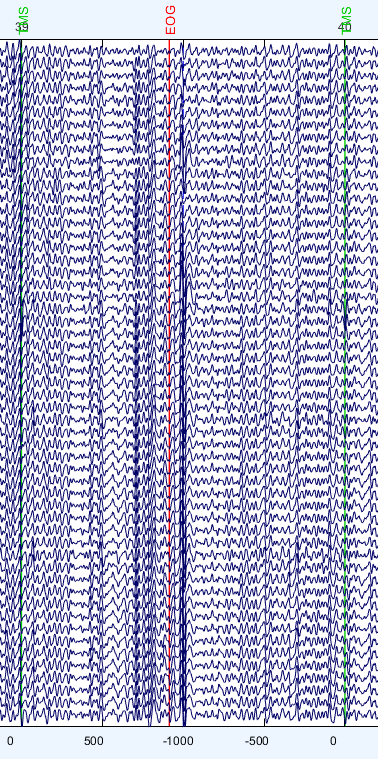
\includegraphics[width=0.9\linewidth, height=10cm]{images/zoom_37eegplot_wavelet_48hzBP.png}
        \caption{Wavelet decomposition.}
        \label{fig:37_eegplot_wavelet}
    \end{subfigure}

\caption{Comparison of EEG channels (epoch 39-40): (a) raw, (b) after fastICA, (c) after wavelet decomposition.}
\label{fig:zoom_37eegplot}
\end{figure}

\subsection{Possible improvements}
\begin{enumerate}
    \item Use more decomposition layers or a different wavelet type, in order too isolate the artifact in 
            a detail level instead of the approximation coefficient as it can lead to lose some TEP information.
            \begin{figure}[H]
                \centering
                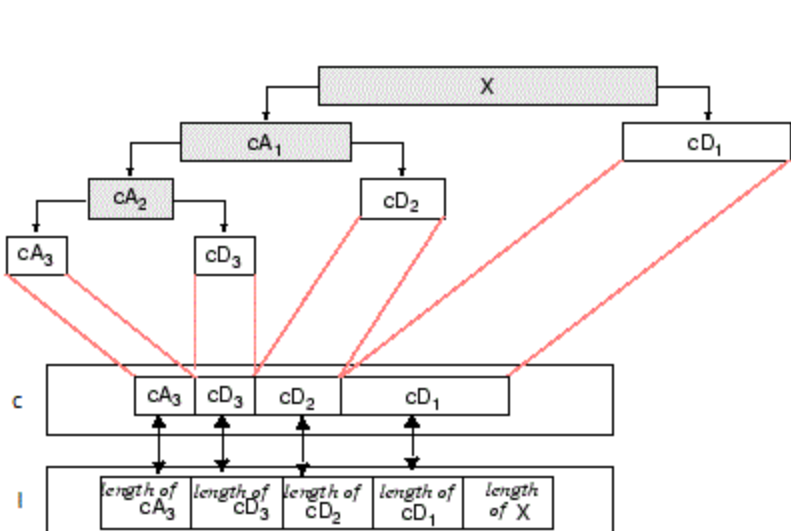
\includegraphics[width=0.6\textwidth]{images/wavedec.png}
                \caption{The image shows that the wavedec matlab function operates by 
                        dividing the signal into approximation coefficients (cA) and detail coefficients (cD). 
                        Then for eache level the approximation coefficients are divided again into
                        approximation coefficients and detail coefficients.
                        }
                \label{fig:wavedec}
            \end{figure}
    \item Use a different method of removing the artifact from the approximation coefficients.

\end{enumerate}


\section{ICA vs Wavelet Decomposition vs EMD}
\subsection{Artifact removal methods}
The following table summarizes the parameters used for the artifact removal methods applied to the TMS-EEG data.
\begin{table}[H]
    \centering
    \begin{tabular}{|l|l|l|}
    \hline
    \multirow{3}{*}{\begin{tabular}[c]{@{}l@{}} \textbf{Wavelet} \\ \textbf{transform}\end{tabular}}               
        & Wavelet type            & Daubechies 4 (db4) \\
        & Levels of decomposition & 12                 \\
        & Detail levels removed   & 7,8,9,10,11,12     \\ \hline \hline
    \multirow{7}{*}{\begin{tabular}[c]{@{}l@{}}\textbf{Empirical} \\ \textbf{Mode} \\ \textbf{Decomposition}\end{tabular}} 
        & Interpolation           & pchip              \\
        & Sift Relative Tolerance & 0.2                \\
        & Max Num IMF             & 5                  \\
        & Sift Max Iterations     & 100                \\
        & Max Number Extrema      & 1                  \\
        & Max  Energy Ratio       & 20                 \\
        & IMFs removed            & 3,4                \\ \hline \hline
    \multirow{4}{*}{\begin{tabular}[c]{@{}l@{}}\textbf{Independent}\\ \textbf{Component}\\ \textbf{Analysis}\end{tabular}} 
        & Approach                & symm               \\
        & g                       & tanh               \\
        & Blink Threshold         & 2.5                \\
        & Move Threshold          & 2                  \\ \hline
    \end{tabular}
\end{table}

\subsection{Results}
The following figures show the results of the comparison between the three artifact removal methods.

\subsubsection{Power Spectral Density (PSD) Comparison}
\begin{figure}[H]
    \centering
    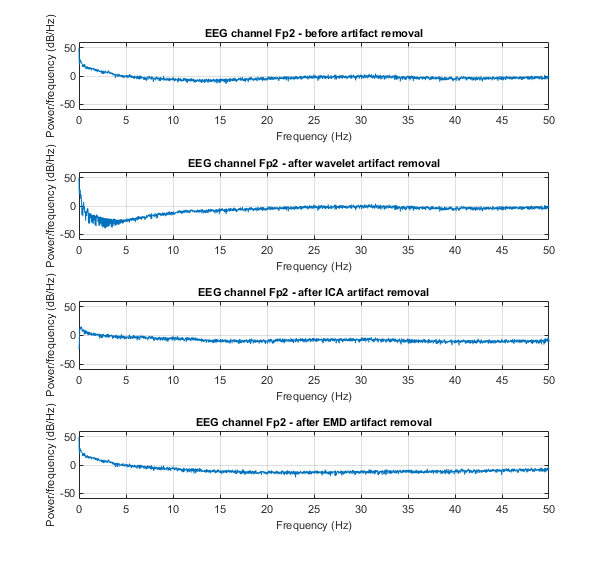
\includegraphics[width=0.75\textwidth]{images/psd_emd.png}
    \caption{PSD graphical comparison before and after artifact removal.}
    \label{fig:psd_emd}
\end{figure}
 
\begin{figure}[H]
    \centering
    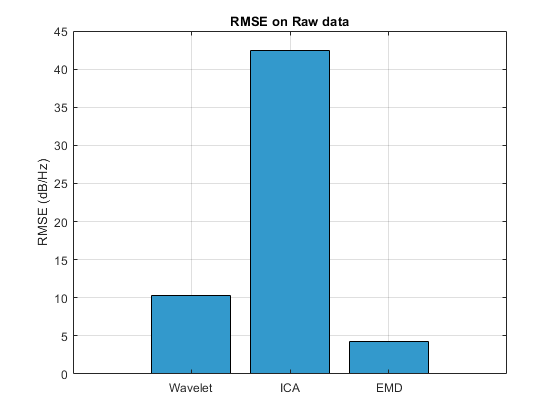
\includegraphics[width=0.8\textwidth]{images/psdrmse_icaemdwave.png}
    \caption{Bar plot of the Root Mean Square Error (RMSE) of the Power Spectral Density (PSD) for each method.}
    \label{fig:psdrmse_icaemdwave}
\end{figure}

\subsubsection{Visual Comparison}

\begin{figure}[htbp]
    \begin{subfigure}{0.24\textwidth}
        \centering
        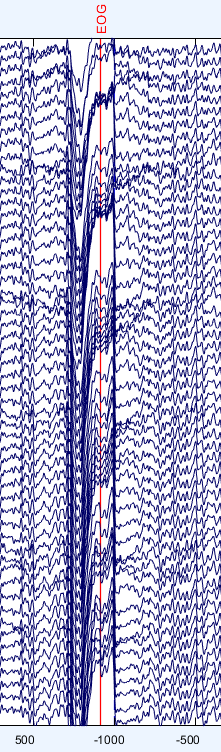
\includegraphics[width=0.9\linewidth, height=10cm]{images/2_visual_comparison/raw_data.png}
        \caption{Raw data.}
        \label{fig:39_eegplot}
    \end{subfigure}
    \begin{subfigure}{0.24\textwidth}
        \centering
        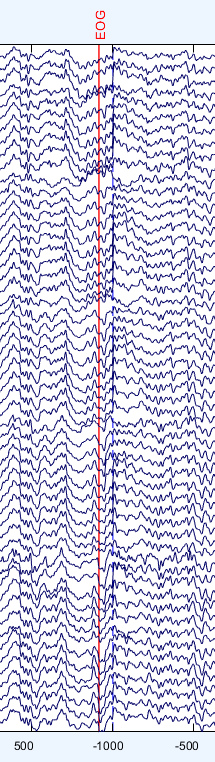
\includegraphics[width=0.9\linewidth, height=10cm]{images/2_visual_comparison/ica.png}
        \caption{FastICA.}
        \label{fig:39_eegplot_ica}
    \end{subfigure}
    \begin{subfigure}{0.24\textwidth}
        \centering
        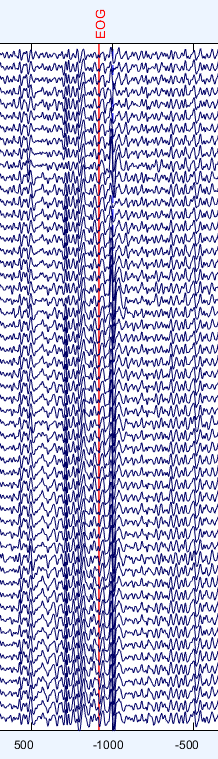
\includegraphics[width=0.9\linewidth, height=10cm]{images/2_visual_comparison/wavelet.png}
        \caption{Wavelet.}
        \label{fig:39_eegplot_wavelet}
    \end{subfigure}
    \begin{subfigure}{0.24\textwidth}
        \centering
        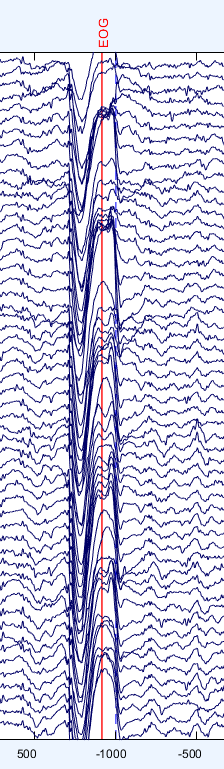
\includegraphics[width=0.9\linewidth, height=10cm]{images/2_visual_comparison/emd.png}
        \caption{EMD.}
        \label{fig:39_eegplot_emd}
    \end{subfigure}
\caption{Comparison of EEG channels (epoch 39-40): (a) raw, (b) after fastICA, (c) after wavelet decomposition, (d) after Empirical Mode Decomposition.}
\label{fig:zoom_39eegplot}
\end{figure}

\subsubsection{Removed signal comparison}
\begin{figure}[H]
    \centering
    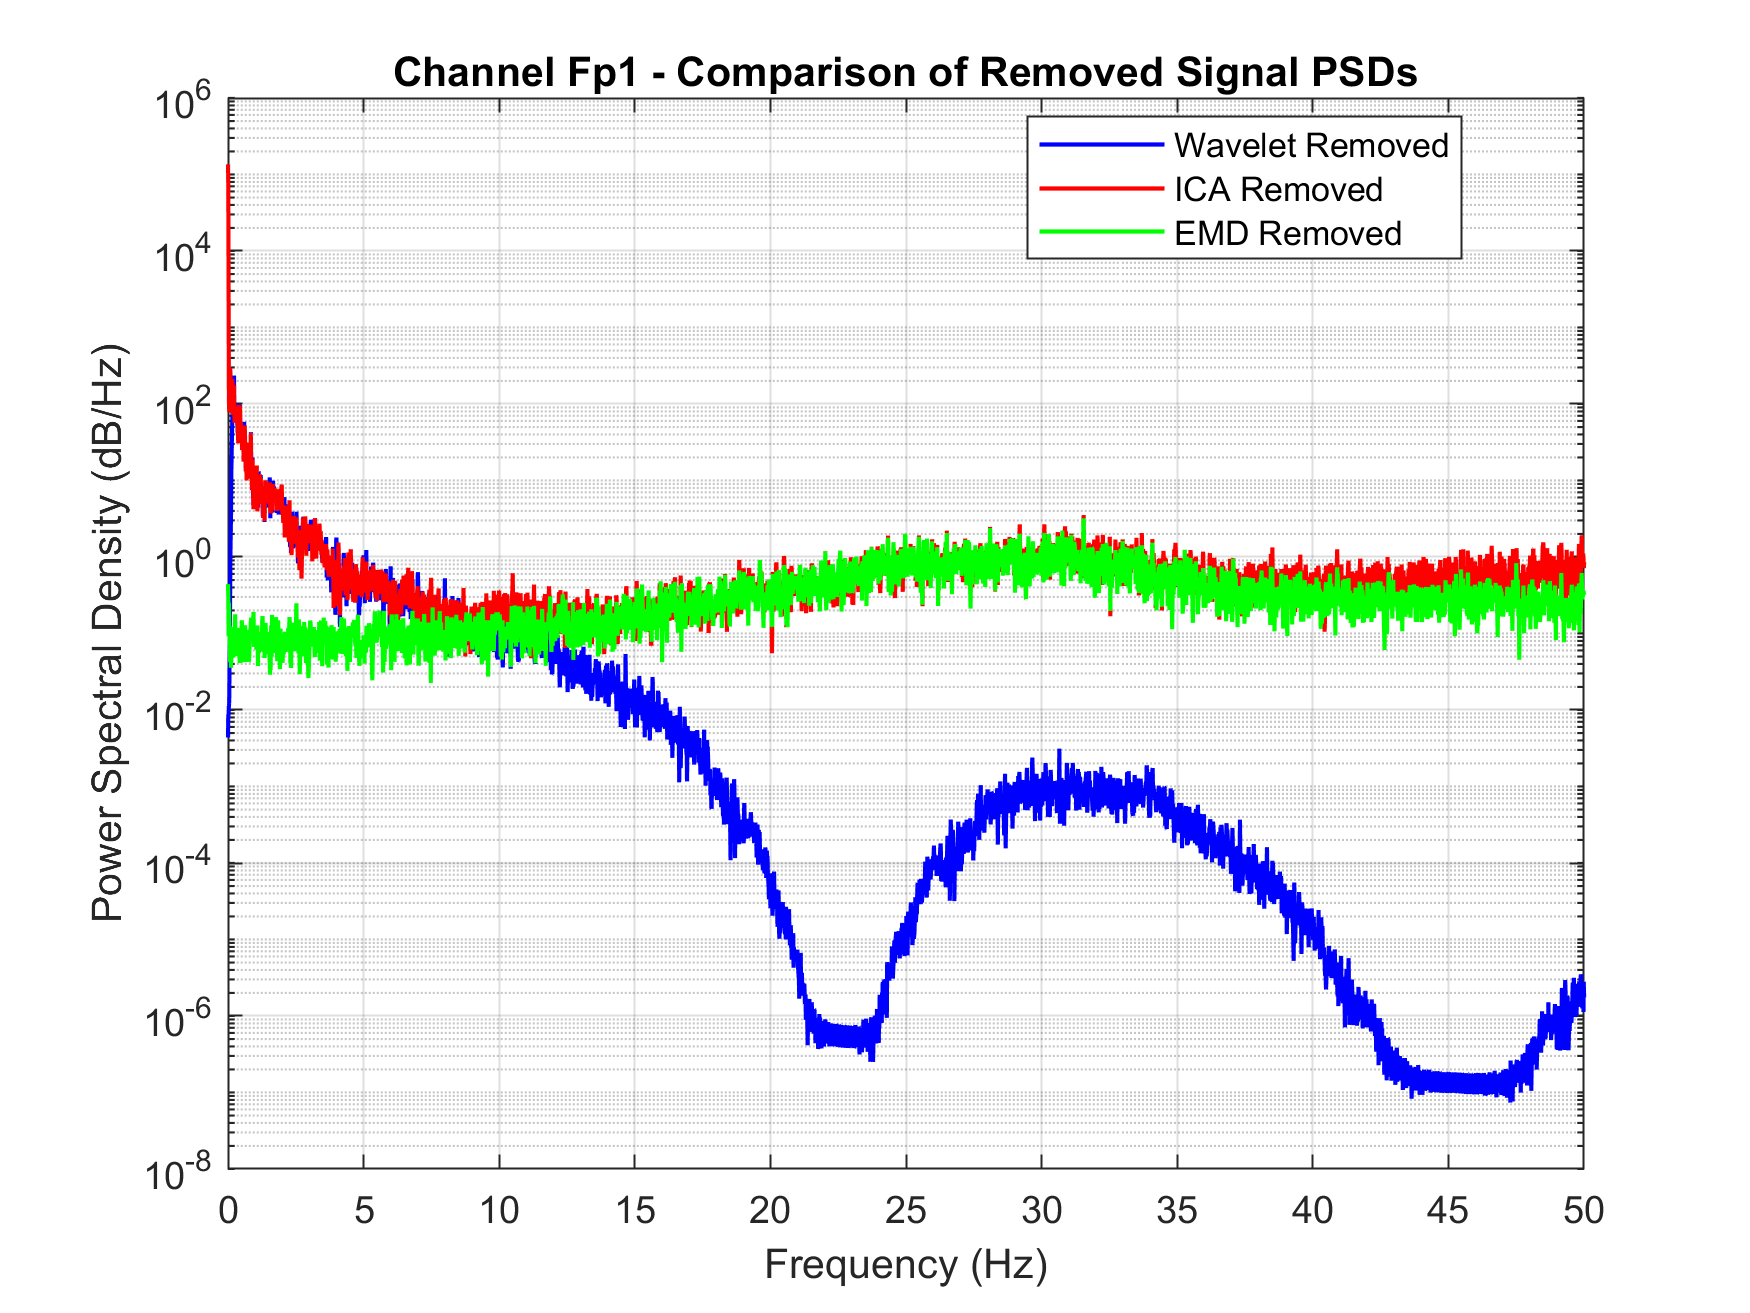
\includegraphics[width=0.8\textwidth]{images/psd_signal_removed.png}
    \caption{PSD of the removed components for each method.}
    \label{fig:psd_signal_removed}
\end{figure}

\begin{figure}[htbp]
    \begin{subfigure}{0.33\textwidth}
        \centering
        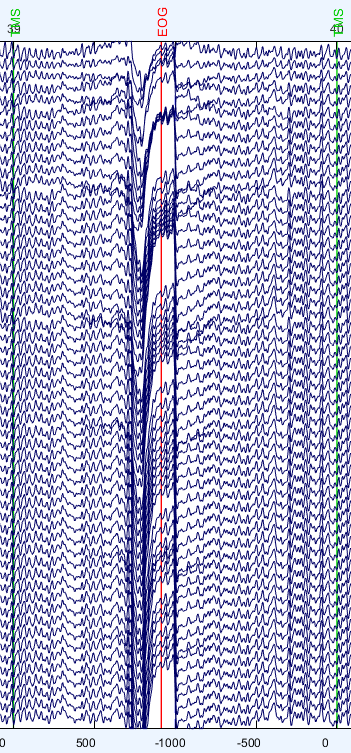
\includegraphics[width=0.99\linewidth, height=9cm]{images/signal_removed/ica_39_(13scale).png}
        \caption{fastICA.}
        \label{fig:39_signal_removed_ica}
    \end{subfigure}
    \begin{subfigure}{0.33\textwidth}
        \centering
        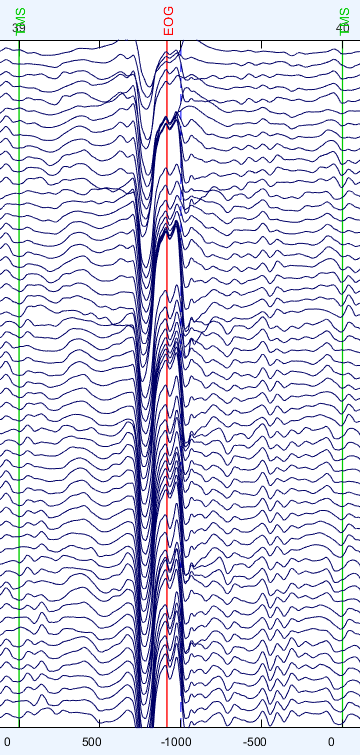
\includegraphics[width=0.99\linewidth, height=9cm]{images/signal_removed/wavelet_39_(13scale).png}
        \caption{Wavelet.}
        \label{fig:39_signal_removed_wavelet}
    \end{subfigure}
    \begin{subfigure}{0.33\textwidth}
        \centering
        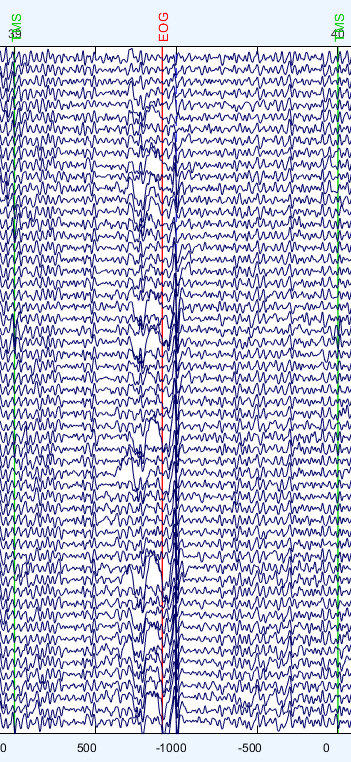
\includegraphics[width=0.99\linewidth, height=9cm]{images/signal_removed/emd_39_(13scale).png}
        \caption{EMD.}
        \label{fig:39_signal_removed_emd}
    \end{subfigure}

\caption{Comparison of the signal removed by the three methods (epoch 39-40): (a) after fastICA, (b) after wavelet decomposition, (c) after EMD.}
\label{fig:39_signal_removed}
\end{figure}

\begin{figure}[htbp]
    \begin{subfigure}{1\textwidth}
        \centering
        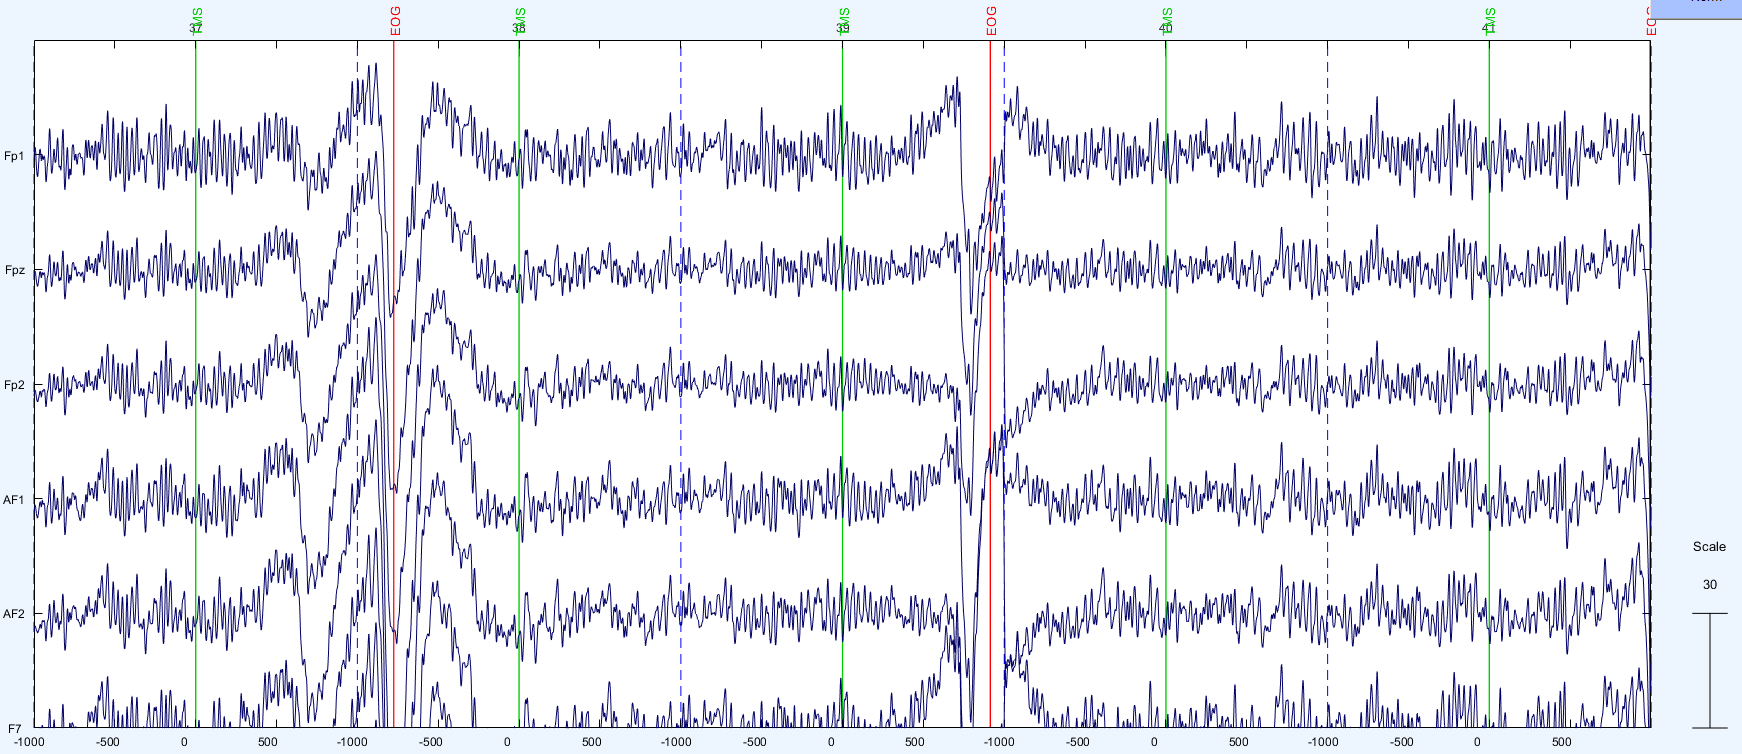
\includegraphics[width=0.99\linewidth, height=6cm]{images/signal_removed/5ch_ica_39.png}
        \caption{fastICA.}
        \label{fig:5ch_39_signal_removed_ica}
    \end{subfigure}
    \begin{subfigure}{1\textwidth}
        \centering
        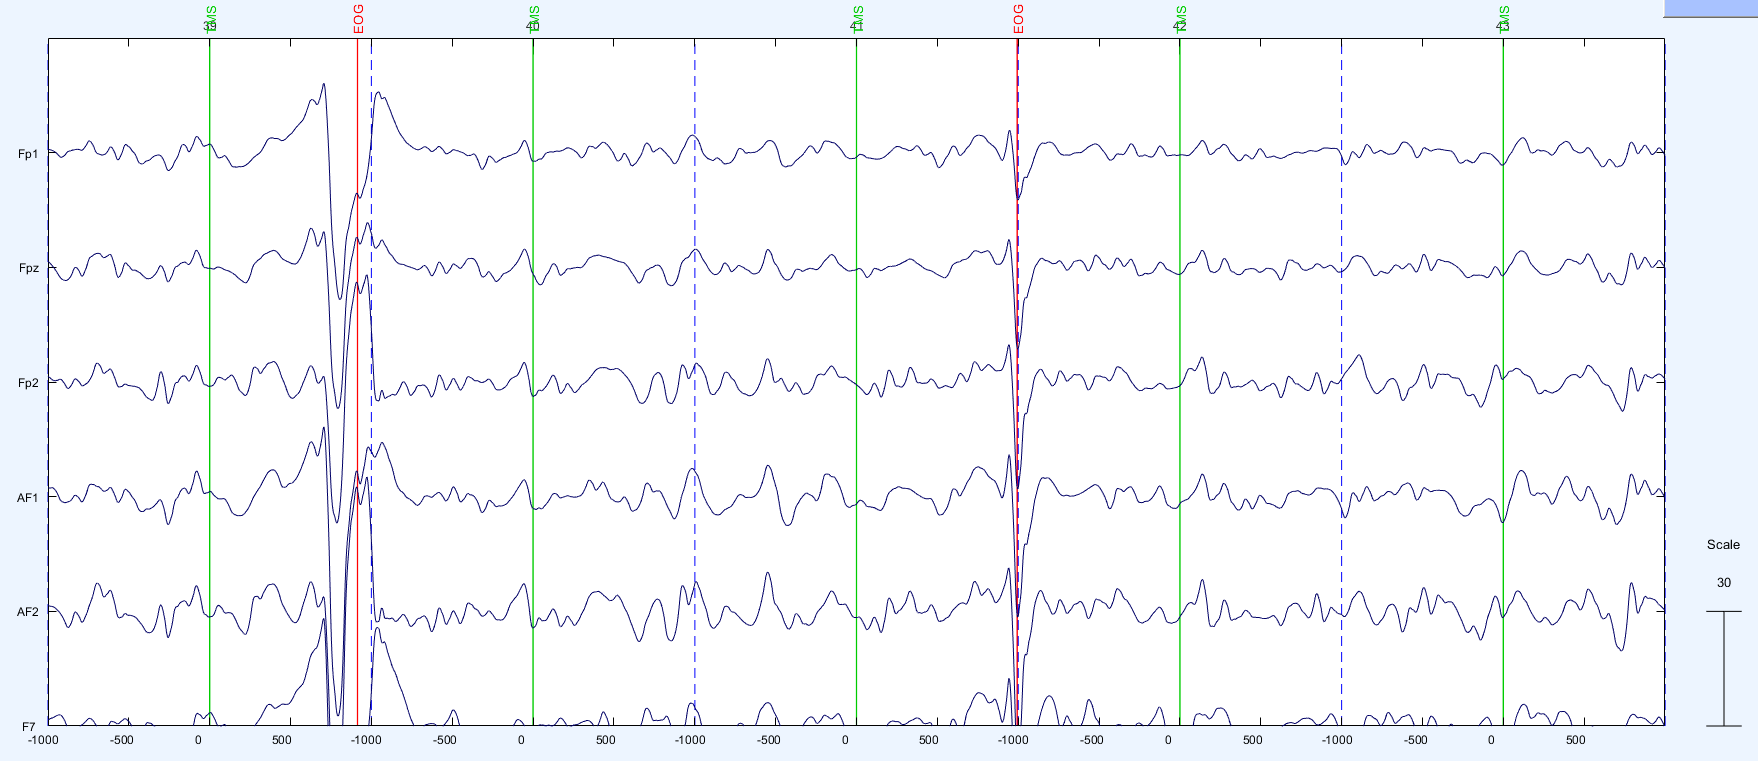
\includegraphics[width=0.99\linewidth, height=6cm]{images/signal_removed/5ch_wavelet_39.png}
        \caption{Wavelet.}
        \label{fig:5ch_39_signal_removed_wavelet}
    \end{subfigure}
    \begin{subfigure}{1\textwidth}
        \centering
        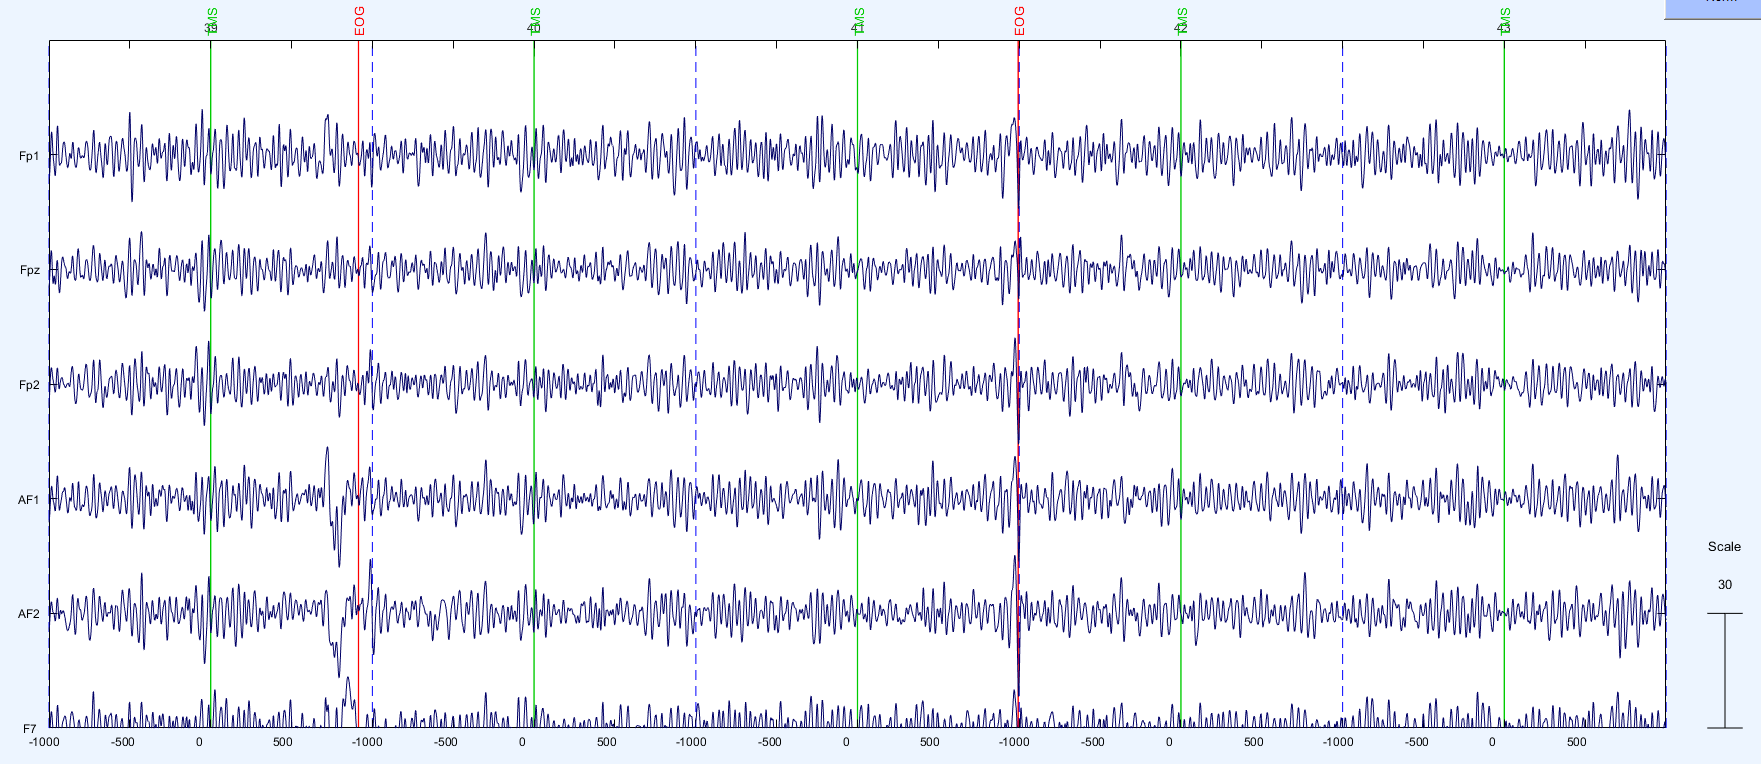
\includegraphics[width=0.99\linewidth, height=6cm]{images/signal_removed/5ch_emd_39.png}
        \caption{EMD.}
        \label{fig:5ch_39_signal_removed_emd}
    \end{subfigure}

\caption{5 channels comparison of the signal removed by the three methods: (a) after fastICA, (b) after wavelet decomposition, (c) after EMD.}
\label{fig:5ch_39_signal_removed}
\end{figure}

\begin{figure}[H]
    \centering
    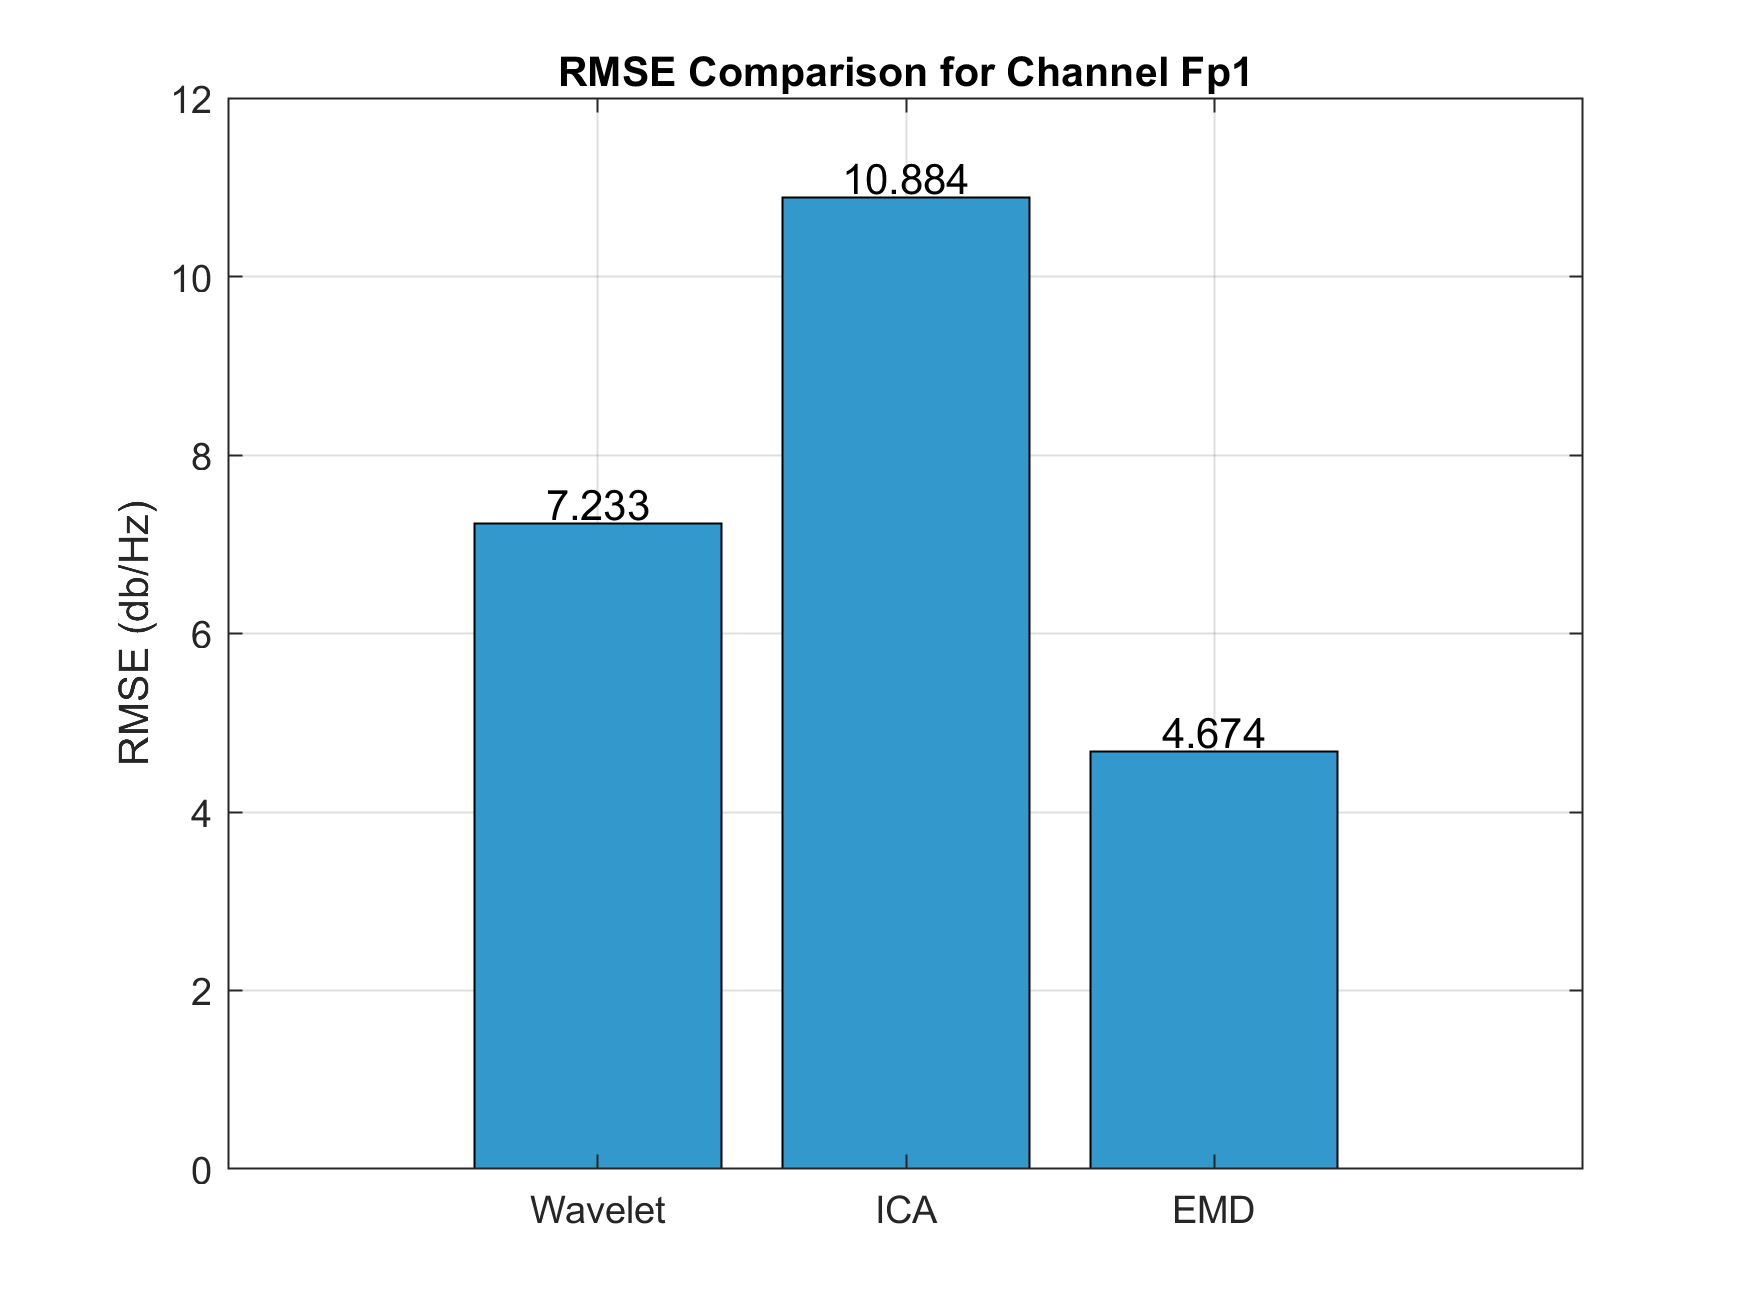
\includegraphics[width=0.8\textwidth]{images/rmse_fp1.png}
    \caption{RMSE has changed, as a result of applying 0.1 Hz hipass filter before every method 
            (before was applied only before fastICA, and was icreasing its rmse).}
    \label{fig:psd_signal_removed}
\end{figure}

\end{document}

\bibliographystyle{alpha}
\bibliography{sample}
